% Compile with latex, then dvisvgm --no-fonts --exact --bbox=min.
\documentclass[tikz,border=5pt]{standalone}
\begin{document}
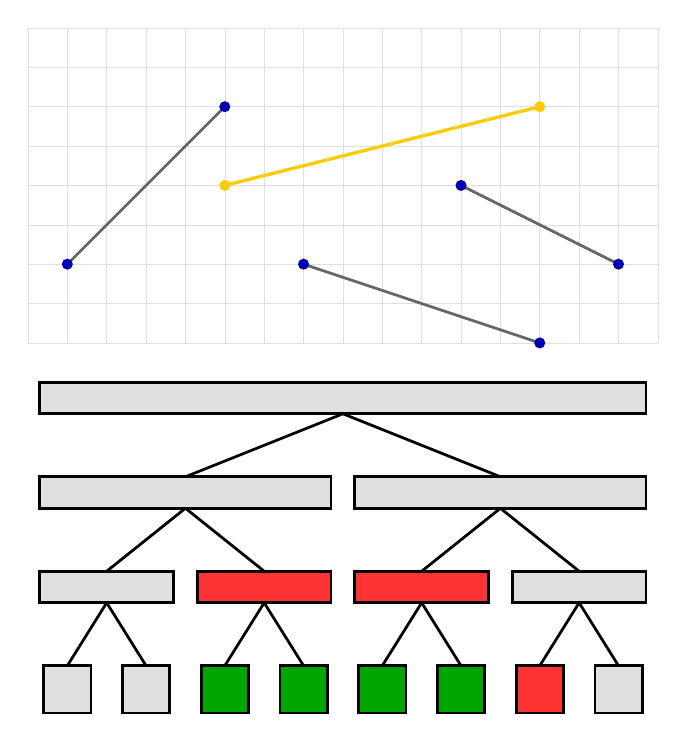
\begin{tikzpicture}[x=1cm,y=1cm,line width=1pt]
  % Eight discrete x positions. The inserted yellow segment covers [3,7].
  \draw[gray!25,very thin] (0.5,0) grid[xstep=0.5,ystep=0.5] (8.5,4);
  \foreach \a/\b/\c/\d in {1/1/3/3,4/1/7/0,6/2/8/1} {
    \draw[gray!80!black] (\a,\b) -- (\c,\d);
    \fill[blue!70!black] (\a,\b) circle (2pt) (\c,\d) circle (2pt);
  }
  \draw[yellow!65!orange,very thick] (3,2) -- (7,3);
  \fill[yellow!65!orange] (3,2) circle (2pt) (7,3) circle (2pt);
  % Tree interval widths align with the plotted x coordinates.
  \foreach \parent/\child in {4.5/2.5,4.5/6.5} {
    \draw (\parent,-0.9) -- (\child,-1.7);
  }
  \foreach \parent/\child in {2.5/1.5,2.5/3.5,6.5/5.5,6.5/7.5} {
    \draw (\parent,-2.1) -- (\child,-2.9);
  }
  \foreach \parent/\child in {1.5/1,1.5/2,3.5/3,3.5/4,5.5/5,5.5/6,7.5/7,7.5/8} {
    \draw (\parent,-3.3) -- (\child,-4.1);
  }
  \draw[fill=gray!25] (0.65,-0.9) rectangle (8.35,-0.5);
  \foreach \a/\b in {0.65/4.35,4.65/8.35} {
    \draw[fill=gray!25] (\a,-2.1) rectangle (\b,-1.7);
  }
  \foreach \a/\b/\color in {0.65/2.35/gray!25,2.65/4.35/red!80,4.65/6.35/red!80,6.65/8.35/gray!25} {
    \draw[fill=\color] (\a,-3.3) rectangle (\b,-2.9);
  }
  \foreach \x/\color in {1/gray!25,2/gray!25,3/green!65!black,4/green!65!black,5/green!65!black,6/green!65!black,7/red!80,8/gray!25} {
    \draw[fill=\color] (\x-0.3,-4.7) rectangle (\x+0.3,-4.1);
  }
\end{tikzpicture}
\end{document}
